\section{Evaluation}\seclabel{Evaluation}

\subsection{A Simple Case Study}
SPADE~\cite{gehani2012spade} is a framework for collecting provenance
information in distributed systems composed of arbitrary black boxes. SPADE
collects provenance information from a variety of sources including operating
system audit logs, network artifacts, LLVM instrumented applications, and
applications dynamically instrumented for taint analysis. These techniques are
the current state of the art in extracting the provenance of arbitrary black
boxes.

In this section, we compare the provenance information produced by SPADE (using
kernel auditing and using LLVM instrumentation) against the provenance
information produced by \fluent{}. To do so, we apply SPADE and \fluent{} to a
trivial workload that consists of a single get request and a single set request
issued against a Redis database. Momentarily, we will see that even for this
trivial workload, \fluent{} produces \watprovenance{} that is orders of
magnitude more succinct than the provenance produced by SPADE.

{\begin{figure}[t]

  \begin{subfigure}[b]{\columnwidth}
    {
      \scriptsize
      \begin{Verbatim}[gobble=8]
        {source:syscall,type:Artifact,hashCode:53bcf1cc966af740e6947b0e9c2a339b,
         id:94,epoch:0,path:/proc/sys/net/core/somaxconn,permissions:0644,
         subtype:file,version:0}
        {source:syscall,type:Artifact,hashCode:581c5ee9cdcf7389575329bf82952436,
         id:95,subtype:memory,version:1,memory address:7f780c538000,size:1000,
         tgid:22694}
        {pid:22694,source:syscall,type:Artifact,hashCode:aacd358e7170deccc70c2f88b52d4cef,
         id:96,epoch:0,subtype:unknown,version:8,fd:1}
        {pid:22694,source:syscall,type:Artifact,hashCode:c86147ac594fd4f80b476a6a928aaf56,
         id:97,epoch:0,subtype:unknown,version:9,fd:1}
        {source:syscall,type:Artifact,hashCode:a38ba1e7456b3e55852c279196a27603,
         id:98,epoch:0,path:/proc/sys/vm/overcommit_memory,permissions:0644,
         subtype:file,version:0}
        {source:syscall,type:Artifact,hashCode:ddc09af7f5ee63ea5d27b62bce4f92e7,
         id:99,subtype:memory,version:2,memory address:7f780c538000,size:1000,tgid:22694}
        {pid:22694,source:syscall,type:Artifact,hashCode:55e22f988b6b65f2114cdaa4e944480d,
         id:100,epoch:0,subtype:unknown,version:10,fd:1}
      \end{Verbatim}
    }
    \caption{Kernel audit provenance}
    \figlabel{SyscallProv}
  \end{subfigure}

  \vspace{0.5cm}

  \begin{subfigure}[b]{\columnwidth}
    {
      \scriptsize
      \begin{Verbatim}[gobble=8]
        {FunctionID:jemalloc_constructor.0.23984,FunctionName:jemalloc_constructor,
         ThreadID:23984,type:Process,hashCode:bf1efff78cc36fca4e34ba0b7bdea49d,id:0}
        {FunctionID:malloc_init_hard_a0_locked.1.23984,FunctionName:
         malloc_init_hard_a0_locked,ThreadID:23984,type:Process,
         hashCode:10a9c5270a6e2f6ea962cd387787b4ec,id:1}
        {FunctionID:je_base_boot.2.23984,FunctionName:je_base_boot,ThreadID:23984,
         type:Process,hashCode:a8210dae28f03bf0cc8f8f43bff1b0ec,id:2}
        {FunctionID:je_malloc_mutex_init.3.23984,FunctionName:je_malloc_mutex_init,
         ThreadID:23984,type:Process,hashCode:833b92e80ae64062350b522d285a08b6,id:3}
        {type:Artifact,hashCode:76c88e33c157de390e9574bf0196b3de,id:4,
         ArgName:mutex,ArgType:%struct.malloc_mutex_s*,ArgVal:0x7fed42d84520}
        {type:Artifact,hashCode:70da28e8a2611657ba8842e198f401db,id:5,ReturnType:i1,
         ReturnVal:0}
        {FunctionID:je_extent_tree_szad_new.4.23984,FunctionName:je_extent_tree_szad_new,
         ThreadID:23984,type:Process,hashCode:b668894d14a1e0f73b5a45ea39208e9f,id:6}
        {type:Artifact,hashCode:3dae7527e64285b9269b2b81a3c3ca9c,id:7,ArgName:rbtree,
         ArgType:%struct.extent_tree_t*,ArgVal:0x7fed42d84548}
      \end{Verbatim}
    }
    \caption{LLVM instrumentation provenance}
    \figlabel{LlvmProv}
  \end{subfigure}
  \caption{SPADE provenance}
  \figlabel{Spade}
\end{figure}
}
{\begin{table}[t]
  \centering
  \caption{SPADE and \fluent{} provenance size}
  \tablabel{ProvSizes}
  \begin{tabular}{ll}
    \toprule
    Tool                         & Number of provenance entries \\\midrule
    SPADE (kernel auditing)      & 1,087 \\
    SPADE (LLVM instrumentation) & 1,118,764 \\
    Fluent                       & 8 \\
    \bottomrule
  \end{tabular}
\end{table}
}

\paragraph{SPADE (Kernel Auditing)}
The Linux kernel includes an auditing subsystem that records security related
events that take place on a system. For example, the auditing subsystem can
intercept and record the syscalls that are issued by processess running on the
system. Thus, the auditing subsystem can record when sockets are opened, when
files are read from or written to, when processes are launched, etc. We
configured SPADE to capture the information produced by this auditing subsystem
and ran our trivial get and set workload. SPADE produced a provenance graph
with 191 vertices and 896 edges. A small sample of the information stored in
the vertices is shown in \figref{SyscallProv}.

This type of kernel audit provenance has two major flaws. The first and most
notable is that it includes a large amount of low-level information that is
difficult to understand. Before a developer can debug with the kernel audit
provenance, they must first have a strong understanding of the various Linux
syscalls. Then, they must understand when and why Redis issues these syscalls,
which requires a deep understanding of Redis' implementation. Second, the
kernel audit provenance doesn't include some vital pieces of information that
are required to understand the workload. Notably, syscalls do not capture
writes to memory, so they do not provide visibility into the fact that our get
request reads from the same memory location as the previous set request.

\paragraph{SPADE (LLVM Instrumentation)}
SPADE can trace the function calls of certain LLVM instrumented executables. We
compiled the Redis server with LLVM instrumentation and integrated it with
SPADE. We did \emph{not} compile the Redis client with LLVM instrumentation, so
SPADE did \emph{not} trace the function calls of the client. We then ran our
simple Redis workload. SPADE produced a provenance graph with 399,916 vertices
and 718,848 edges! A sample of the information stored in these vertices is
shown in \figref{SyscallProv}.

This provenance has two shortcomings. The first is immediate; the provenance
includes an overwhelming amount of information. A single set and get request
produced over a million combined vertices and edges. If the Redis server
processed a modest ten transactions per second for one minute, it would produce
over half a \emph{billion} combined vertices and edges. Worse, interpreting
this provenance requires a deep understanding of the underlying Redis
implementation. Second, when an executable is compiled with LLVM
instrumentation, it's execution is significantly slowed because every function
invocation requires the executable to report provenance information to the
SPADE server.

\paragraph{\fluent{}}
Finally, we ran our workload with \fluent{}. \fluent{} produced eight data
entries: a get and set request and response on both the Redis client and the
Redis server. This is four orders of magnitude more succinct that the SPADE
provenance produced by LLVM instrumentation. Moreover, applying Redis'
\watprovenance{} specification to the get request, it returns the previous set
request and nothing else. We summarize these findings in \tabref{ProvSizes}

\subsection{\WatProvenance{} Specifications}
% file system , read and write byte ranges, 88 python
% redis, set, del, append, incr, decr, incrby, decrby, strlen, get 30 lines sql;
% s3, cp, cat, ls, rm, rb, 200 lines python
% zookeeper, get set create ls, 70 lines sql

\subsection{Shim Overheads}
We now measure the performance overheads of \fluent{} shims. \fluent{} shims
increase the latency and reduce throughput of black boxes for two reasons.
First, there is a latency overhead in proxying messages to and from a black
box. Second, there is a latency overhead in persisting the messages to a
relational database.  Some of these overheads can be avoided---e.g., \fluent{}
shims buffer messages in memory and only periodically persist them to a
relation database---but some overhead is unavoidable.

In this subsection, we measure the overheads introduced by \fluent{} shims for
two black boxes: Redis and Amazon S3. We do so with the following three step
experiment.
\begin{enumerate}
  \item
    We measure the throughput of each black box when it is not wrapped in a
    \fluent{} shim.
  \item
    We measure the throughput of each black box when it is wrapped with a
    \fluent{} shim that does not persist any messages. This ``partial shim''
    incurs the overheads of proxying messages but not the overheads of
    persisting them.
  \item
    We measure the throughput of each black box when it is wrapped with a fully
    functional \fluent{} shim that periodically persists messages to a
    relational database. Unlike the partial shim, This ``full shim'' incurs all
    of the overheads of a \fluent{} shim.
\end{enumerate}

To measure the throughput of Redis, we have a single client perform small two
byte set requests to a single key for five seconds. To measure the throughput
of S3, we have a single client create, read, and delete 25 objects in a single
bucket. Each object is 1 KB. We run clients, shims, and black boxes on
t2.xlarge instances on Amazon EC2. We colocate shims with their black boxes,
but otherwise place clients and black boxes on different instances within the
same availability zone. We repeat each throughput measurement twenty times.
Box plots of these throughput measurements are shown in \figref{Shims}.

\begin{figure}[ht]
  \centering
  \begin{subfigure}[b]{\columnwidth}
    \centering
    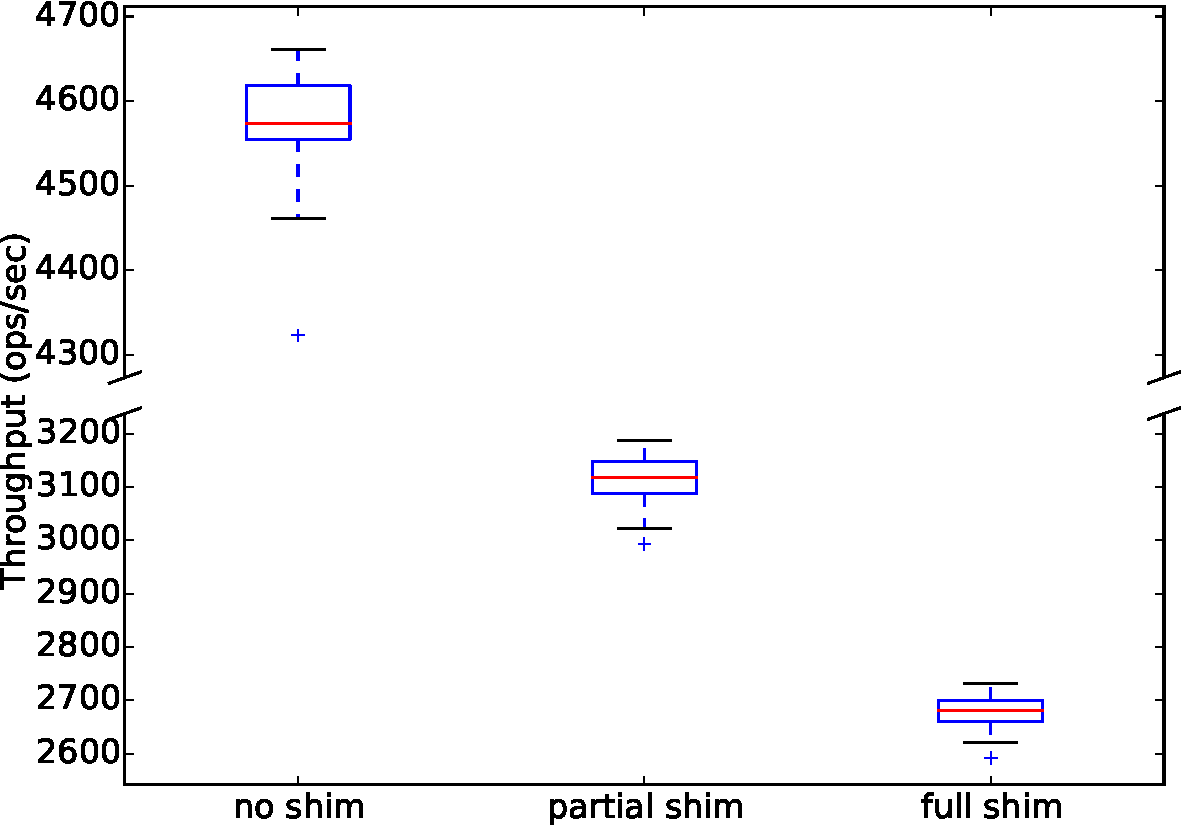
\includegraphics[width=0.8\columnwidth]{figures/redis_shim.pdf}
    \caption{Redis throughput}
    \figlabel{RedisShim}
  \end{subfigure}

  \begin{subfigure}[b]{\columnwidth}
    \centering
    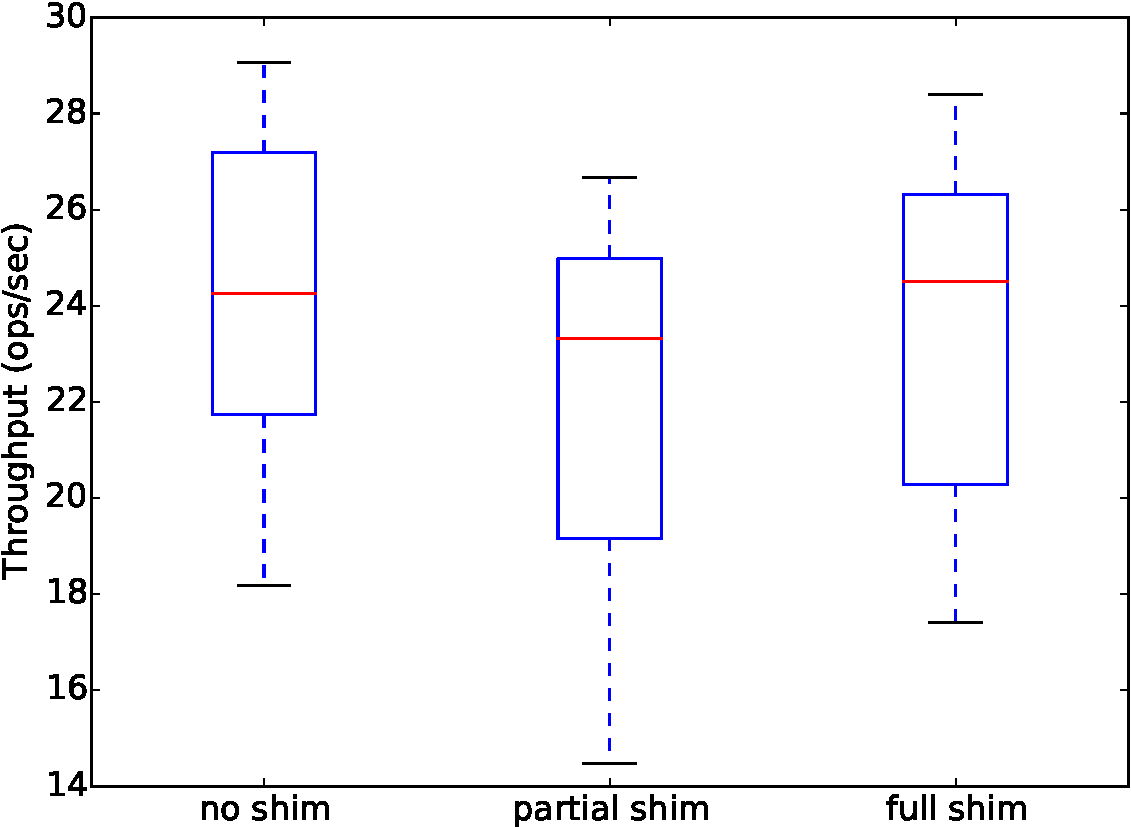
\includegraphics[width=0.8\columnwidth]{figures/s3_shim.pdf}
    \caption{S3 throughput}
    \figlabel{S3Shim}
  \end{subfigure}%
  \caption{The overheads of \fluent{} shims}
  \figlabel{Shims}
\end{figure}

% (4566.224999999999  , 332.309657849422)
% (3111.4139999999998 , 225.28554831590938)
% (2676.5609999999997 , 144.54921507915557)
Redis averages a throughput of 4566 set requests per second (with standard
deviation 322) when not wrapped with a \fluent{} shim. When it is wrapped with
a \fluent{} shim that does not persist messages, the throughput drops to an
average of 3111 set requests per second (with a standard deviation of 225).
When Redis is wrapped with a fully functional shim, its throughput drops to
2676 set request per second. These large decreases in throughput are expected.
Redis is a lightweight system, and the time it takes to service a single set
request is very low. Thus, even small overheads can significantly decrease
throughput.  While these overheads are fundamental to our shim-based approach,
they will likely decrease as we continue to optimize \fluent{}'s prototype
implementation.

% (24.222414999999998 , 14.674786717547207)
% (22.34917           , 15.440412655172143)
% (23.572789999999998 , 15.308642281338997)
Unlike Redis, S3's throughput is relatively unaffected by the overheads of the
shims. Without any shim, S3 averages a throughput of 24.22 operations per
second (with standard deviation 14.67). This throughput drops only slightly to
22.35 operations per second (with standard deviation 15.44) and 23.58
operations per second (with standard deviation 15.31) when S3 is wrapped with a
partial and full\fluent{} shim respectively. In contrast to Redis, S3
sacrifices low latency and high throughput for availability. Thus, the small
overheads introduced by the shims are largely negligible.
